%%%%%%%%%%%%%%%%%%%%%%
% NASTAVENÍ FEKT.TEX %
%%%%%%%%%%%%%%%%%%%%%%

% Pokud následující řádky zakomentujete, na titulní straně se nezobrazí.

% Nadpis dokumentu (kód předmětu)
\newcommand{\name}{MPC-PDA}
% Podnadpis dokumentu (název předmětu)
%\newcommand{\subname}{}
% Seznam autorů
\newcommand{\authors}{Studenti IBE}
% Seznam korektorů
%\newcommand{\corrections}{}
% Popis dokumentu
\newcommand{\docdesc}{Příprava na zkoušku 2023}
% Zařazení dokumentu (studijní program)
\newcommand{\docgroup}{Informační bezpečnost, FEKT VUT}
% Odkaz
\newcommand{\docurl}{https://github.com/BeziCZ/MPC-PDA}

% Přepsáním argumentu na 'true' zapnete balíček 'minted' pro sázení kódu.
% Pro jeho použití lokálně musíte mít v systému dostupný Python 3, python
% knihovnu 'minted' a PDFLaTeX musíte spouštět s argumentem '-shell-escape'.
% Místo něj můžete použít prostředí 'lstlisting'.
\newcommand{\docminted}{false}


%%%%%%%%%%%%%%%%%%%%
% OBECNÉ NASTAVENÍ %
%%%%%%%%%%%%%%%%%%%%

\newcommand{\fekttexversion}{2.0}

\documentclass[
    % Velikost základního písma je 12 bodů
    12pt,
    % Formát papíru je A4
    a4paper,
    % Oboustranný tisk
    twoside,
    % Záložky a metainformace ve výsledném PDF budou v kódování unicode
    unicode,
]{article}

% Kódování zdrojových souborů
\usepackage[utf8]{inputenc}
% Kódování výstupního souboru
\usepackage[T1]{fontenc}
% Podpora češtiny
\usepackage[czech]{babel}

% Geometrie stránky
\usepackage[
    % Horní a dolní okraj
    tmargin=25mm,
    bmargin=25mm,
    % Vnitřní a vnější okraj
    lmargin=30mm,
    rmargin=20mm,
    % Velikost zápatí
    footskip=17mm,
    % Vypnutí záhlaví
    nohead,
]{geometry}

% Zajištění kopírovatelnosti a prohledávanosti vytvořených PDF
\usepackage{cmap}
% Podmínky (pro použití v titulní straně)
\usepackage{ifthen}

%%%%%%%%%%%%%%%
% FORMÁTOVÁNÍ %
%%%%%%%%%%%%%%%

% Nastavení stylu nadpisů
\usepackage{sectsty}
% Formátování obsahů
\usepackage{tocloft}
\setcounter{tocdepth}{1}
% Odstranění mezer mezi řádky v seznamech
\usepackage{enumitem}
\setlist{nosep}
\setitemize{leftmargin=1em}
\setenumerate{leftmargin=1.5em}
\renewcommand{\labelitemi}{--}
\renewcommand{\labelitemii}{$\circ$}
\renewcommand{\labelitemiii}{$\cdot$}
\renewcommand{\labelitemiv}{--}
% Sázení správných uvozovek pomocí '\enquote{}'
\usepackage{csquotes}
% Vynucení umístění poznámek pod čarou vespod stránky
\usepackage[bottom]{footmisc}
% Automatické zarovnání textu k předcházení vdov a parchantů
\usepackage[defaultlines=3,all=true]{nowidow}
% Zalomení části textu pokud není na současné stránce dost místa
\usepackage{needspace}
% Nastavení řádkování
\usepackage{setspace}
\onehalfspacing
% Změna odsazení odstavců
\setlength{\parskip}{1em}
\setlength{\parindent}{0em}

% Bezpatkové sázení nadpisů
\allsectionsfont{\sffamily}
% Změna formátování nadpisu a podnadpisů v Obsahu
\renewcommand{\cfttoctitlefont}{\Large\bfseries\sffamily}
\renewcommand{\cftsubsecdotsep}{\cftdotsep}

% Použití moderní/aktualizované sady písem
\usepackage{lmodern}

%%%%%%%%%%%
% NADPISY %
%%%%%%%%%%%

\usepackage{titlesec}

\titlespacing*{\section}{0pt}{10pt}{-0.2\baselineskip}
\titlespacing*{\subsection}{0pt}{0.2\baselineskip}{-0.2\baselineskip}
\titlespacing*{\subsubsection}{0pt}{0.2\baselineskip}{-0.2\baselineskip}
\titlespacing*{\paragraph}{0pt}{0pt}{1em}

%%%%%%%%%%
% ODKAZY %
%%%%%%%%%%

% Tvorba hypertextových odkazů
\usepackage[
    breaklinks=true,
    hypertexnames=false,
]{hyperref}
% Nastavení barvení odkazů
\hypersetup{
    colorlinks,
    citecolor=black,
    filecolor=black,
    linkcolor=black,
    urlcolor=blue
}

%%%%%%%%%%%%%%%%%%%%%%%%%%%
% OBRÁZKY, GRAFY, TABULKY %
%%%%%%%%%%%%%%%%%%%%%%%%%%%

% Vkládání obrázků
\usepackage{graphicx}
\usepackage{subfig}
% Nastavení popisů obrázků, výpisů a tabulek
\usepackage{caption}
\captionsetup{justification=centering}
% Grafy a vektorové obrázky
\usepackage{tikz}
\usetikzlibrary{shapes,arrows}
% Složitější tabulky
\usepackage{tabularx}
\usepackage{multicol}

% Sázení osamocených float prostředí v horní části stránky
\makeatletter
\setlength{\@fptop}{0pt plus 10pt minus 0pt}
\makeatother

% Vynucení vypsání floating prostředí pomocí \FloatBarrier
\usepackage{placeins}

% Rámečky
\usepackage{mdframed}

%%%%%%%%%%%%%%
% MATEMATIKA %
%%%%%%%%%%%%%%

% Sázení matematiky a matematických symbolů ('\mathbb{}')
\usepackage{amsmath}
\usepackage{amssymb}
% Sázení fyzikálních veličin
\usepackage{siunitx}

%%%%%%%%%%%%%%%%%
% ZDROJOVÉ KÓDY %
%%%%%%%%%%%%%%%%%

% Sazba zdrojových kódů
\usepackage[formats]{listings}
% Přepnutí prostředí 'code' do režimu výpisu kódu
\newenvironment{code}{\captionsetup{type=listing}}{}

\lstset{
    basicstyle=\small\ttfamily,
    numbers=left,
    numberstyle=\tiny,
    tabsize=4,
    columns=fixed,
    showstringspaces=false,
    showtabs=false,
    keepspaces,
}

% Balíček 'minted' budeme používat pouze pokud je jeho hodnota nastavena na 'true'
\providecommand{\docminted}{false}
\ifthenelse{\equal{\docminted}{true}}
{
    % Sazba zdrojových kódů
    \usepackage[newfloat]{minted}
    % Nastavení barev 'minted' kódů
    \usemintedstyle{pastie}
}
{
    % \docminted není 'true', nic neprovádíme
    % Pokud je v dokumentu 'minted' prostředí, dokument se nepodaří přeložit.
}

%%%%%%%%%%%%%%%%%%%
% VLASTNÍ PŘÍKAZY %
%%%%%%%%%%%%%%%%%%%

\newcounter{todo}
\newcommand{\TODO}[1]{%
    \addtocounter{todo}{1}%
    \textcolor{red}{%
    \textbf{\sffamily\small{TODO \thetodo}%
    \ifthenelse{\equal{#1}{}}{}{:}%
    } %
    #1%
    }%
}

%%%%%%%%%%%
% TITULKA %
%%%%%%%%%%%

\newcommand{\titulka}{
    \vspace*{2em}
    \begin{center}
        \ifthenelse{\isundefined{\name}}{}{{\Huge \bfseries \name{}}}

        \ifthenelse{\isundefined{\subname}}{}{{\huge \bfseries \subname{}}}

        \vspace*{2em}

        \ifthenelse{\isundefined{\docdesc}}{}{{\Large \docdesc}}

        \vspace*{1em}

        \ifthenelse{\isundefined{\docgroup}}{}{\docgroup}

        \ifthenelse{\isundefined{\docurl}}{}{\url{\docurl}}
    \end{center}

    \vfill

    \ifthenelse{\isundefined{\authors}}{}{\authors{}}
    \ifthenelse{\isundefined{\corrections}}{}{\\\small (korektury \corrections{})}

    {}{\small \today}
    \\{\small FEKT.tex \fekttexversion{}}

    \thispagestyle{empty}
    \newpage
}

%%%%%%%%%%%%
% DOKUMENT %
%%%%%%%%%%%%

\begin{document}

\titulka{}

\tableofcontents
\thispagestyle{empty}

\setcounter{page}{0}

\section{Teorie složitosti}
\subsection{Druhy složitosti}

\subsubsection{Polynomiální vs exponenciální složitost}
\begin{itemize}
    \item Polynomiální složitost
    \begin{itemize}
        \item S délkou vstupu (\(n\)) roste čas potřebný k vyřešení lineárně (\(n^x\)). Tudíž čas potřebný k řešení roste propocionálně, ale ne exponenciálně.
        \item Lze je řešit bez potřeby vysoké výpočetní síly.
    \end{itemize}
    \item Exponeciální složitost
    \begin{itemize}
        \item Lze je řešit efektivně bez velkého výpočetního výkonu pouze pro malé vstupy
        \item Čas potřebný pro řešení roste s počtem vstupů \(n\) exponenciálně \(x^n\)
    \end{itemize}
\end{itemize}

\subsubsection{Třídy složistoti}
\begin{itemize}
    \item P
    \item NC
    \item NP
    \item NP-Complete 
    \item NP-Hard
    \item \#P
    \item PSPACE
    \item NL
    \item EXP
    \item EXPSPACE
\end{itemize}

\subsubsection{Třída P}
Spadají do ní problémy, které je možné řešit v polynomiálním čas na deterministickém turingově stroji. Spadají sem například problémy jako je nalezení nekratší
cesty nebo nalezení kostry grafu.
\subsubsection{Třída NC}
Podmožina P, která obsahuje problémy, které se dají řešit v polylogaritmickém paralelním čase na polynomiálním počtu procesorů.\\
Problém se vstupem délky \(n\) je v NC pokud existují konstanty \(k\) a \(c\) takové, že platí \(O(k \cdot log^cn)\) pak je možné vyřešit problém za \(O(log^cn)\)
na \(O(n^k)\) paralelních procesorech.\\
P je pro určení míry efektivity algoritmů při sekvenčním provádění a NC je pro určení míry efektivity při paralelním provádění.

\subsubsection{Třída NP}
Obsahuje problémy, které je možné řešit v polynomiálním čase na nedeterministickém turingově stroji.\\
\subsubsection{Třída NP-Complete}
Podmožina NP, která obsahuje nejtěžší problémy v NP. Problém x je NP-Complete pokud je možné za polynomiální transformovat NP problém y na
problém x. Nebylo pro ně nalezeno polynomiální řešení, ale dokázáno, že řešení existuje. Na deterministickém turingově stroji je možné je řešit pouze za
exponenciální čas. Pokud by bylo nalezeno řešení v polynomiálním čase pak by to znamenalo, že P=NP, protože nalezení řešení pro jeden NP-Complete problém
znamená nalezení řešení pro všechny NP-Complete problémy.\\
Do NP-C spadá například barvení grafů, Knapsack problem(problém batohu), 3-partition problem(rozdělení množiny čísel na trojice se stejným součtem).

\subsubsection{Třída NP-Hard}
Obsahuje problémy, které jsou alespoň tak těžké jako jsou NP-Complete problémy, ale zároveň se neví jestli patří do NP. Problém x je NP-Hard pokud se na něj
redukuje problém y který je ze třídy NP-Complete za polynomiální čas. Existují také problémy, které jsou NP-Hard, ale ne NP-Complete,
například problém zastavení turingova stroje nebo problém splnitelnosti booleovské formule, Travelling salesman problem.

\subsubsection{Třída \#P}
Neřeší hledání řešení problémů, ale řeší hledání počtu možných řešení problému ze třídy NP. Tudíž problémy v této třídě musí být alespoň stejně těžké jako
daný NP problém. 

\subsubsection{Třída PSPACE}
Problémy, které lze řešit na deterministickém turingově stroji s polynomiálním objemem paměti. V této třídě nezáleží na času, který je problém řešen.
Například hledání hodnoty pozice na nekonečně velké hrací ploše šachů.

\subsubsection{Třída NL}
Třída, která obsahuje rozhodovací algorimy řešitelké na nedeterministickém turingově stroji v logaritmickým objemem paměti. Díky tomu, že třída L(Logarithmic
space) je podmnožinou třídy P, tak z toho plyne, že jakýkoliv problém v NL je možné vyřešit pomocí deterministického turingova stroje s polynomiálním množstvím
paměti. Obsahuje podmnožinu problémů NL-Complete, které jsou nejtěžší problémy v NL a jakýkoliv problém z NL na ně lze redukovat. Jejím příkladem je například
problém dostupnosti v orientovaných grafech.

\subsubsection{Třída EXP}
Označována také jako EXPTIME. Problémy řešitelné na sekvenčních počítačích v exponenciálním čase. Obsahuje také EXP-Complete problémy

\subsubsection{EXPSPACE}
Stejné jako EXP, ale místo času řeší paměť

\subsection{Algoritmická řešení}

\subsection{Aproximační algortimy}
\subsubsection{Genetické algoritmy}
Založeny na procesu evoluce, řešení jsou reprezentovány vektory řešení. Jedna buňka tohoto vektoru se nazývá gen, reprezentovány pomocí čísel nebo jiných datových
struktur podle problému. Základní operace v GA, mutace je změna jednotlivého genu, crossover je vyměňování genů mezi jednotlivci. Pok křízení a mutaci se generuje
nová populace. Hledání nejlepších kandidátů pomocí fitness funkce.

\subsubsection{Genetické programování}
Reprezentace pomocí stromu. Stejný princip jako genetické algorimy mutace je však změna části podstromu, křízení je prohození podstromu mezi různými stromy. 
Obsahuje funce a terminály, kde terminály jsou prvky v listech stomu, které nemají vlastní potomky. 

\subsubsection{Optimalizace rojem částic}
Každá částice se pomocí aktualizace své pozice v prostoru (2D, 3D) snaží najít optimální řešení problému. Každá z částic si udržuje informace o vlastní poloze, nejlepší poloze
kterou kdy dosáhla(kokální optimum) a nejlepší poloze nalezenou kteroukoliv částicí v roji(globální optimum). 
\begin{gather*}
    X(t+1) = X(t) + V(T+1)\\
    V(t+1) = W\cdot V(t) + C_1\cdot rand()X(X_{pbest}-X(t)) + C_2\cdot rand()X(X_{gbest}-X(t))
\end{gather*}
kde \(V(t)\) je rychlost v čase \(t\), \(X(t)\) je pozice v čase \(t\), \(W\) je váha, \(C_1\) a \(C_2\) jsou učící a akcelerační faktory, \(rand()\) je náhodné
číslo v intervalu inkluzivním intervalu mezi 0 a 1 s normálním rozdělením, \(X_ {pbest}\) je lokální optimum a \(X_{gbest}\) je globální optimum. \\
Obecně algorimus funguje tak, že dokud není splněna podmínka terminace 

\subsubsection{Optimalizace mravenčí kolonií}
Jednotliví mravenci reprezentují částečná řešení. Mravenci postupují prostorem a tím krok po kroku budují řešení. Jejich pohyb je založen na feromonech a na 
stochastických parametrech. Poté se vyhledá lokální minimum. Nakonec se aktualizují feromony pozitivně pro ty cesty, které jsou dobré a negativně pro cesty, které
jsou špatné. Toto proces se opakuje dokud není splněna ukončující podmínka.\\
Narozdíl od ostatních aproximačních algoritmů nepoužívá křízení, ale pouze mutaci. Jednotlivci jsou reprezentováni pomocí páru číselných vektorů \(\mathbf{v} =
(\mathbf{x},\boldsymbol{\sigma})\). Kde \(\mathbf{x}\) bod ve stavovém prostoru reprezentovaný vektorem čísel a \(\boldsymbol{\sigma}\) je vektor směrodatné 
odchylky. Mutace pak probíhá:\\
\begin{gather*}
    \mathbf{x}^{t+1} = \mathbf{x}^t + N(0, \boldsymbol{\sigma})
\end{gather*}
Kde N je náhodné číslo z funce gaussova normálního rozdělení se směrodatnou odchylkou \(\boldsymbol{\sigma}\) a průměrem 0
\section{Genetické algoritmy vs Genetické programování}

\begin{itemize}
    \item GA i GP spadají do skupiny Evolučních algoritmů
    \item GP je (prý z několika zdrojů, co jsem našel idk) speciální případ GA, kdy se dá použít hierarchická struktura pro vytváření samostatných \uv {programů}, které hledají řešení problému. GA jsou obecnější a univerzálnější pro optimalizační problémy.
    \item Reprezentace vstupu: U GA se jedná o vektory (chromozomy), které reprezentují každý jednu proměnnou v problému. U GP je to strom, který reprezentuje hierarchickou strukturu primitiv (plus, minus atd.) a terminálů (proměnné $x$,$y$, konstanty atd.).

\end{itemize}
\section{Grafy - algoritmy}
\subsection{Detekce cyklů}
\begin{itemize}
    \item Cyklický graf - graf obsahuje aspoň jeden cyklus
    \item Pokud neobsahuje, je acyklický
    \item \textbf{DAG} - Directed Acyclic Graph
    \item U nesměrovaných grafů lze použít DFS, graf je acyklický v případě že DFS nevrátí již navštívěný uzel
    \item DFS nelze použít u směrovaných grafů, zde iterativě odstraňujeme uzly s nulovým in-degree. V případě, že skončíme s jedním uzlem, jedná se o DAG
\end{itemize}
\subsection{Maďarský algoritmus}
Algoritmus pro hledání maximální shody - max. matching.

Postup:
\begin{itemize}
    \item Problém reprezentujeme maticí
    \item Nejmenší hodnotu v řádků odečteme od všech hodnot v řádku
    \item Nejmenší hodnotu v sloupci odečteme od všech hodnot v sloupci
    \item V matici škrtneme řádky a sloupce tak, aby by vyškrtnuté všechny nuly, a byl použit nejnižší možný počet těcho čar
    \item V případě že se množství čar= množství řádků matice, máme optimální řešení
    \item Pokud nemáme optimální řešení, vezmeme nejmenší neškrtnutou hodnotu v každém řádku a přičteme ji k ke každému průsečíku čar.
    
\end{itemize}
\subsection{Node2Vec}
algoritmus pro generování vektorových reprezentací uzlů v grafu. Rámec node2vec se učí nízkorozměrné reprezentace uzlů v grafu pomocí random walks grafem počínaje cílovým uzlem
\TODO{no idea, v prezentacích o tom nic pořádně není}
\subsection{Strongly Connected Components}
Silně propojený komponent grafu je maximálně silně propojený subgraf
\subsubsection{Kosrajův algoritmus}
Postup:
\begin{itemize}
    \item DFS pro vypočítání opouštějícího času pro každý uzel
    \item Výpočet inverzního grafu
    \item DFS na inverzním grafu, začínáme uzelm s nejvyšší hodnotou opuštění uzlu.
    \item Navštívené uzly ukládáme do setu SCC
    \item Po dokončení iterace je komponent uložen, zvolí se další uzel a nacházejí se další komponenty
    \item Algoritmus je ukončen po navštívení všech uzlů
\end{itemize}
\subsubsection{Tarjanův algoritmus}
\begin{itemize}
    \item Jednotlivé uzly uchovávají hodnoty "index" a "low"
    \item Postupně procházíme graf, iteruje se index a low
    \item po cyklu nastavíme low na nejnižší dosažitelné low předchozích uzlů
    \item Pokud index=low, uzel je kořen SCC
    \item Uzly se stejným low tvoří SCC
\end{itemize}
\subsection{Izomorfismus}
Grafy jsou izomorofní v případě, že jsou mezi nimi zachovány jejich základní vlastnosti - cesty, podgrafy. Tedy existuje bijekce která zobrazuje jeden graf na druhý.
Pro ověření se používá \textbf{Ullmanův algoritmus:}
\begin{itemize}
    \item Vytvoříme matici sousednosti pro oba grafy a permutační matici - obsahuje pouze jednu 1 v každém sloupci a řádku
    \item Matici sousednosti jednoho grafu vynásobíme nejprve s permutační maticí, a výsledek poté znovu vynásobíme s transponovanou permutační maticí
    \item Pokud se výsledek rovná matici sousednosti druhého grafu, jsou izomorfní
    \item V opačném případě zkusíme jinou variaci permutační matice, připadně po vyčerpání všech možností perm. matice grafy nejsou izomorfní
\end{itemize}
\section{Neuronky}
\subsection{Hloubka sítě, výpočet, princip}

Hloubka neuronové sítě definuje počet vrstev neuronů, které nn obsahuje.

\subsection{Princip konvolučních sítí}
Konvoluční neuronové sítě narozdíl od ostatních přivádí jiné vrstvy než plně propojené. Tyto sítě jsou založeny na kombinování různých typů vrstev, plně
propojených, konvolučních, max-pooling. Můžou se používat pro různé dimenze dat 1D pro time-series nebo zpracování hlasu, 2D pro zpracování obrazu, 3D pro data z
MRI nebo CT.\\
\subsubsection{Konvoluční vrstva}
Vrstva je založena na konvoluci vstupních dat s konvolučním kernelem. Tento kernel je reprzentován maticí vah, která se posouvá po vstupních datech. Pomocí těchto
kernelů se provádí často operace pro zjednodušení vstupních dat, například detekce hran v obraze. Konvoluce jako taková je matematická operace, která funguje na 
pricipu násobení části vstupu maticí vah a součet výsledku těchto součinů. Pokud máme matici X vstupu 3x3 a kernel K velikosti 3x3 pak bude výsledek konvoluce následující:\\
\begin{align*}
    c = x_{00}\cdot k_{00} + x_{01}\cdot k_{01} + x_{02}\cdot k_{02} + ... + x_{33}\cdot k_{33}
\end{align*}
Vedlejší efekt konvoluce je ten, že zmenšuje vstup a to podle velikosti konvolučního kernelu. Z toho důvodu se často přidává ohraničení 0 tak aby vstupní data
zůstala stejné velikosti.\\
\begin{figure}[ht]
    \centering
    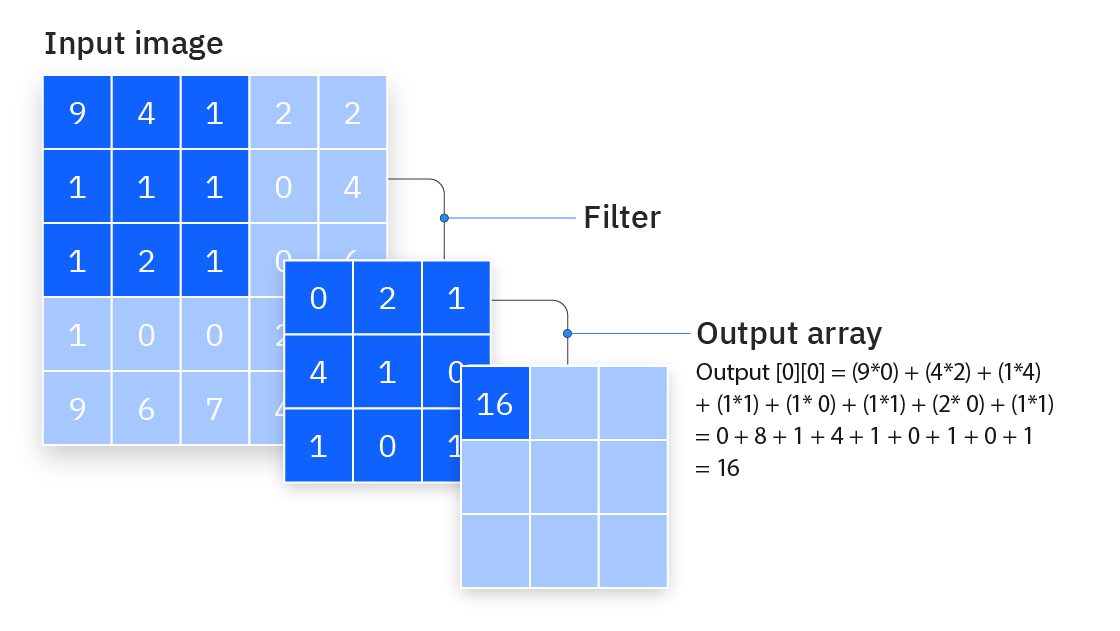
\includegraphics[scale = 0.25]{images/iclh-diagram-convolutional-neural-networks.png}
\end{figure}
\subsubsection{Max Pooling vrstva}
Její účel je zmenšení vstupu pro jednodušší zpracování a zárovenň zachování nejdůležitější informace z oblasti. Stejně jako koncvoluční vrstva používá kernel
pro procházení vstupu. Avšak místo sumy bere pouze největší hodnotu z oblasti přes kterou se kernel posouvá.\\
\begin{figure}[ht]
    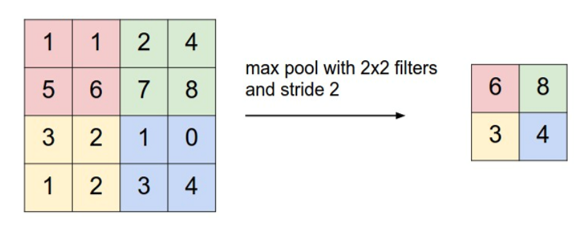
\includegraphics[scale=0.7]{images/MaxPooling.png}
\end{figure}

\subsubsection{Flatten vrstrva}
Používá se po dokončení práce konvolučních a max pooling vrstev pro transformaci dat z matice do vektoru aby mohly být data zpracovány plně propojenými vrstvami. 

\subsubsection{Augmentace dat}
Používá se pro zvýšení různorodosti datasetu. Přidává další data pomocí transformací dat známých.
U obrazu sem patří posuny, rotace, zrcadlení, úpravy kontrastu, jasu, atd. U zvuku například přidání šumu do pozadí, posun tóniny.

\subsubsection{Transfer learning}
Využití toho, že již existují velké sítě, které jsou již natrénované na obřích datasetech a my si doděláme k tomuto modelu jenom klasifikátor.

\subsection{Rekurentní neuronky}
Rekurentní nn používají cykly a faktorem je zde i čas.
Zpracovávají sekvence dat na sekvence výstupů. Narozdíl od klasický NN mají paměť, jejich vnitřní stav označovaný \(h(t)\) je použit pro operaci s dalším vstupem.\\
\begin{figure}[ht]
    \centering
    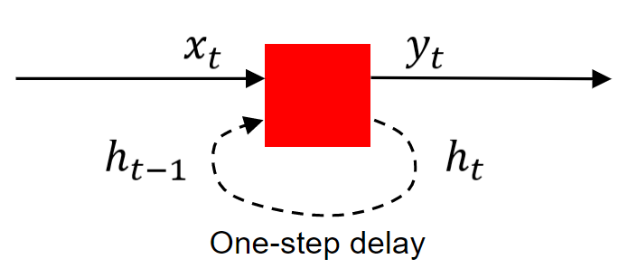
\includegraphics[scale = 0.5]{images/RNN.png}
\end{figure}

\subsubsection{LSTM}
Long Short Term Memory. Pokročilá varianta RNN. Má mnohem složitěší buňku, která je založena na používání bran(gates) pro kontrolu toku informací. LSTM buňka má
4 stavy zpracování:
\begin{enumerate}
    \item Zapomene nepotřebnou historii
    \item Uloží relevantní části nové informace
    \item Pomocí předchozích 2 kroků aktualizuje vnitřní stav
    \item Generuje výstup
\end{enumerate}

\section{QLearning}
\subsection{Princip}
Model-free reinforcement learning algoritmus k zjištění hodnoty akce v konkrétním stavu.
\begin{figure}[h!]
    \centering
    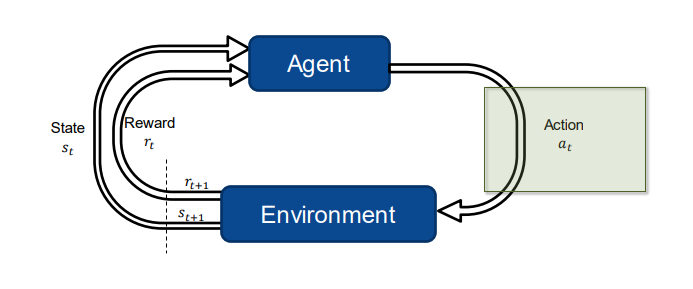
\includegraphics[width=0.5\linewidth]{images/qlearn.png}
    \caption{Q-Learning princip}
    \label{fig:enter-label}
\end{figure}
Základní požadavky:
\begin{itemize}
    \item Prostředí se nemění
    \item Počet stavů a akcí je konečný
    \item Odměny jsou omezené
    \item Rychlost učení se snižuje navštívením párů stav-akce
    \item Exploration metoda garantuje nekonečné navštěvování všech dvojic stav-akce v nekonečné training periodě
\end{itemize}
Nelze vždy zvolit akci s nejvyšší Q hodnotou - Q-funkce je ze začátku neotpimální, je nutno zkoumat možnosti dokud není fce optimální.
Používá se metoda $\epsilon$-hungry, kde se s určitou šancí vykoná náhodná akce, tato pravděpodobnost se postupně snižuje. Agent tedy buď provádí naučenou akci, nebo náhodnou.

\subsection{QLearning vs Sarsa}
Sarsa je on policy algoritmus, používá akci zvolenou současnou policy. Soustředí se na akce které jsou skutečně použity a učí se z následků vlastních rozhodnutí
Q-Learning je off policy, používá greedy approach k naučení se Q-value. SLeduje nejlepší možné akce v každé situaci a učí se z nich.

\section{AI}
\subsection{3 podmínky obecné AI}
\begin{itemize}
    \item Kombinatorická generalizace: Hlavní chybějící požadavek pro obecnou AI a klíčový aspekt vývoje AI. Schopnost skládání nových struktur ze známých stavebních bloků. \uv{Nekonečné využití konečných prostředků}. Noty do skladby. Písmena na slova. Slova do vět.  
    \item Relační zdůvodnění: Základní charakteristika inteligence. Schopnost vidět smysluplné spojení/vzorce mezi objekty (Časové vztahy, prostorové vztahy\dots). 
    \item Relační indukční zaměření: Vybírání co nejvalidnější relace pro vyřešení dané otázky.

\end{itemize}
\subsection{Člověk vs funkce AI}
(tady absolutně nemám tušení, co tím myslí a v přednášce jsem to nikde neviděl a jedinej rozdíl je snad ta kombinatorická generalizace, že AI není schopná vidět jakoukoliv jinou relaci, než tu, na kterou se naučila)

\subsection{Předávání zpráv v grafu (princip)}
\TODO{Jsou asi 3 typy v poslední přednášce, zjistit, jestli potřebuje všechny a chtělo by to asi obrázek + tam někde dělá matici záměn a netuším, jestli to chce jako popsat celé}

Graf $H_t$ předá zprávu na graf $H_{t+1}$. Nejspíš potřebuje jen tu první, protože ta se asi obecně použije podle toho, jak je napsaná ta prezentace, ale má tam 3 typy.
\subsubsection{Average ze sousedů a hodnoty sama sebe}
Hodnoty na jednotlivých uzlech se vypočítají jako jako aritmetický průměr sousedních hodnot a samotného uzlu.
\subsubsection{Average ze sousedů bez hodnoty sama sebe}
Hodnoty na jednotlivých uzlech se vypočítají jako aritmetický průměr sousedních hodnot, ale bez samotného uzlu.
\subsubsection{Suma sousedů}
Hodnoty na jednotlivých uzlech se vypočítají jen jako suma sousedních uzlů.



\end{document}
